\input{preamble.tex}

\title{Observability Data Engineering}
\subtitle{A Story About Math, Four Golden Signals, and Business Intelligence}
\institute{DevOps Observability Architect}
\author{Jack Neely\\ jjneely@gmail.com}

\date{\today}

\newcommand{\hcancel}[1]{%
    \tikz[baseline=(tocancel.base)]{%
        \node[inner sep=0pt,outer sep=0pt] (tocancel) {#1};
        \draw[lightblue, very thick] (tocancel.south west) -- (tocancel.north east);
    }%
}%

\begin{document}

%% Introduction, Title
\maketitle

%% In the Before Time Lightning Talk
%% Consultant work
\begin{frame}
    \frametitle{Monitorama PDX 2019: How to know if something is ``up''}
    \begin{tikzpicture}[remember picture,overlay]
        %%\node[at=(current page.center)] {
        %%    \includegraphics[width=10cm]{img/lightning-2019.png}
        %%};
    \end{tikzpicture}
\end{frame}

\begin{frame}
    \frametitle{As a DevOps Observability Architect...}

    \emph{What do I monitor?}

    Google SRE's \hcancel{Four} Five Golden Signals
    \begin{description}
        \item[Health] Pods are Running and Healthy
        \item[Traffic] Counter of Units of Work
        \item[Errors] Counter of Units of Work with Exceptions
        \item[Latency] Timer of the distribution of latencies for each Unit of Work
        \item[Saturation] When Pods be scaled up or down
    \end{description}

    Remember: \alert{There are FIVE lights!}
\end{frame}

\begin{frame}
    \frametitle{As a DevOps Observability Architect...}

    The \hcancel{Four} Five Golden Signals is knowing before the customers do.

    \pause
    \begin{quote}
        \emph{We need to set alerts for these super special customers.}
    \end{quote}

    Well, if we set our Histograms correctly and record maximum values we will
    be able to tell when...

    \pause
    \begin{quote}
        \emph{When a customer calls we need to be able to verify the error
            they encountered.  We'll need a high cardinally solution.}
    \end{quote}

    Umm...those aren't metrics.  How heavily are you sampling your traces?

    \pause
    \begin{quote}
        \emph{Jack, we're an Enterprise!}
    \end{quote}
\end{frame}

\begin{frame}
    starship goes here
\end{frame}

\frame[standout]{Traffic}

%% Count Units of Work
%% Why Counting monotonoically matters like a network device

\begin{frame}
    \frametitle{Why Counters Work}

    \begin{quote}
         Systems based in cumulative monotonic sums are naturally simpler, in
         terms of the cost of adding reliability. When collection fails
         intermittently, gaps in the data are naturally averaged from
         cumulative measurements.  -- OpenTelemetry Data Model
    \end{quote}

    Most Accurate: Incremented in discrete whole numbers.  Never misses an
    event.

    Synchronization Primitive: Allows for multiple observers.

    Low Overhead: Easy implementation.  No copying or recalling previous
    values.

    Fundamental: \textbf{Position!}

    %% https://www.researchgate.net/publication/3849082_Monotonic_counters_A_new_mechanism_for_thread_synchronization
\end{frame}

\begin{frame}
    \frametitle{Remembering Physics}
    \begin{columns}
        \begin{column}{0.33\textwidth}
            Position
            \resizebox{\columnwidth}{!}{\begin{tikzpicture}[/pgf/declare function={f=3*x^3-6*x^2+2*x-1;}]
\begin{axis}[
    domain=0:10,
    ymax=2500,
    samples=100,
    axis lines=middle,
    xticklabel=$t_{\pgfmathprintnumber{\tick}}$
]
\addplot [thick] {f};
\end{axis}
\end{tikzpicture}
}
        \end{column}
        \begin{column}{0.33\textwidth}
            Velocity
            \resizebox{\columnwidth}{!}{\begin{tikzpicture}[/pgf/declare function={f=9*x^2 - 12*x + 2;}]
\begin{axis}[
    domain=0:10,
    ymax=2500,
    samples=100,
    axis lines=middle,
    xticklabel=$t_{\pgfmathprintnumber{\tick}}$
]
\addplot [thick] {f};
\end{axis}
\end{tikzpicture}
}
        \end{column}
        \begin{column}{0.33\textwidth}
            Acceleration
            \resizebox{\columnwidth}{!}{\begin{tikzpicture}[/pgf/declare function={f=18*x - 12;}]
\begin{axis}[
    domain=0:10,
    ymax=2500,
    samples=100,
    axis lines=middle,
    xticklabel=$t_{\pgfmathprintnumber{\tick}}$
]
\addplot [thick] {f};
\end{axis}
\end{tikzpicture}
}
        \end{column}
    \end{columns}
    \note[item]{Spike detection}
\end{frame}

\begin{frame}[fragile]
    \frametitle{Counting Caveats: Riemann Sums}
    \note[item]{How to aggregate Counters}
    \begin{columns}
        \begin{column}{0.5\textwidth}
            \resizebox{\columnwidth}{!}{\pgfplotsset{
    integral segments/.code={\pgfmathsetmacro\integralsegments{#1}},
    integral segments=10,
    integral/.style args={#1:#2}{
        ybar interval,
        domain=#1+((#2-#1)/\integralsegments)/2:#2+((#2-#1)/\integralsegments)/2,
        samples=\integralsegments+1,
        x filter/.code=\pgfmathparse{\pgfmathresult-((#2-#1)/\integralsegments)/2}
    }
}

%% https://math.dartmouth.edu/opencalc2/cole/lecture8.pdf
%%\begin{tikzpicture}[/pgf/declare function={f=0.1*x^2+1;}]
\begin{tikzpicture}[/pgf/declare function={f=3*x^3-6*x^2+2*x-1;}]
\begin{axis}[
    domain=0:10,
    samples=100,
    axis lines=middle,
    xticklabel=$t_{\pgfmathprintnumber{\tick}}$
]
\addplot [
    red,
    fill=red!50,
    integral=0:10
] {f};
\addplot [thick] {f};
\end{axis}
\end{tikzpicture}
}
        \end{column}
        \begin{column}{0.5\textwidth}
\begin{lstlisting}
interval: 5m
rules:
- record: labels:http_server_requests:rate5m
  expr: >
    sum by (service, namespace, status) (
      rate(http_server_requests_seconds_count{}[5m])
    )
\end{lstlisting}

Integrate and Build Ratio:
            \begin{lstlisting}
1 - (
  sum_over_time(
    sum without (status) (
      labels:http_server_requests:rate5m{
        status=~"5..", service="..."})[7d:5m]
  ) * 300 /
  sum_over_time(
    sum without (status) (
      labels:http_server_requests:rate5m{
        service="..."})[7d:5m]
  ) * 300
)
            \end{lstlisting}
        \end{column}
    \end{columns}
\end{frame}

\frame[standout]{Errors}

%% Count Units of Work that fail or create an exception
%% How you CPU metrics are wrong

\begin{frame}[fragile]
    \frametitle{Measuring CPU Usage Over Time}

    How do you measure CPU usage of a process?
    \begin{enumerate}[label=\alph*.]
        \item Jiffies
        \item Percentages
        \item Seconds a Process is in the Running State
        \item All of the above
    \end{enumerate}
\end{frame}

\begin{frame}
    \frametitle{Nyquist-Shannon Sampling Theorem}
    \begin{figure}[!h]
        \centering
        \begin{tikzpicture}[/pgf/declare function={f=sin(deg(0.5*pi*x+0.25*pi));g=sin(deg(pi*x));}]
\begin{axis}[
    width=\textwidth,
    height=0.6\textheight,
    domain=0:10,
    samples=500,
    axis lines=middle,
    xticklabel=$t_{\pgfmathprintnumber{\tick}}$
]
\addplot [red, thick] {g};
    \addplot [mark=*, only marks] coordinates {(0.5,1) (4.5, 1) (8.5,1) (1.83, -0.5) (3.16,-0.5) (5.83,-0.5) (7.16,-0.5) (9.83,-0.5)};
\end{axis}
\end{tikzpicture}

    \end{figure}
    $$ Scrape Interval > 2f $$
\end{frame}
\begin{frame}
    \frametitle{Nyquist-Shannon Sampling Theorem}
    \begin{figure}[!h]
        \centering
        \input{nyquist-shannon2.tex}
    \end{figure}
    $$ Scrape Interval > 2f $$
\end{frame}

\frame[standout]{Latency}

%% Latency: Timers and Distributions -- Why averages are horrible and
%% Anscombe's Quartet. Understanding Gamma Distributions.

\begin{frame}
    \frametitle{Anscomb's Quartet}
    \begin{columns}
        \begin{column}{0.3\textwidth}
            \begin{center}
                \begin{tabular}{ c c }
                    \multicolumn{2}{c}{\textbf{Summary Statistics}} \\
                    \hline
                    $N$ & $11$ \\
                    $\mu\{x_1..x_n\}$ & $9.0$ \\
                    $\mu\{y_1..y_n\}$ & $7.5$ \\
                    $\sigma\{x_1..x_n\}$ & $3.16$ \\
                    $\sigma\{y_1..y_n\}$ & $1.94$ \\
                    $r^2$ & $0.67$
                \end{tabular}
            \end{center}
        \end{column}
        \begin{column}{0.7\textwidth}
            \begin{figure}[!h]
                \centering
                \subfloat{%
\begin{tikzpicture}[/pgf/declare function={f=0.5001*x+3.0001;}]
\begin{axis}[
    %%width=\textwidth,
    height=4.5cm,
    xmax=20,
    xmin=0,
    ymin=0,
    ymax=13,
    samples=100,
    domain=0:20,
    axis lines=middle,
    yticklabels={,,},
    xticklabels={,,},
    mark size=1pt,
]
    \addplot [mark=*, only marks] table[x=x1, y=y1] {anscombs.dat};
    \addplot [red] {f};
\end{axis}
\end{tikzpicture}%
}%
%
\subfloat{%
\begin{tikzpicture}[/pgf/declare function={f=0.5000*x+3.0009;}]
\begin{axis}[
    %%width=\textwidth,
    height=4.5cm,
    xmax=20,
    xmin=0,
    ymin=0,
    ymax=13,
    samples=100,
    domain=0:20,
    axis lines=middle,
    yticklabels={,,},
    xticklabels={,,},
    mark size=1pt,
]
    \addplot [mark=*, only marks] table[x=x2, y=y2] {anscombs.dat};
    \addplot [red] {f};
\end{axis}
\end{tikzpicture}%
}

\subfloat{%
\begin{tikzpicture}[/pgf/declare function={f=0.4997*x+3.0025;}]
\begin{axis}[
    %%width=\textwidth,
    height=4.5cm,
    xmax=20,
    xmin=0,
    ymin=0,
    ymax=13,
    samples=100,
    domain=0:20,
    axis lines=middle,
    yticklabels={,,},
    xticklabels={,,},
    mark size=1pt,
]
    \addplot [mark=*, only marks] table[x=x3, y=y3] {anscombs.dat};
    \addplot [red] {f};
\end{axis}
\end{tikzpicture}%
}%
%
\subfloat{%
    \begin{tikzpicture}[/pgf/declare function={f=0.4999*x+3.0017;}]
\begin{axis}[
    %%width=\textwidth,
    height=4.5cm,
    xmax=20,
    xmin=0,
    ymin=0,
    ymax=13,
    samples=100,
    domain=0:20,
    axis lines=middle,
    yticklabels={,,},
    xticklabels={,,},
    mark size=1pt,
]
    \addplot [mark=*, only marks] table[x=x4, y=y4] {anscombs.dat};
    \addplot [red] {f};
\end{axis}
\end{tikzpicture}%
}

            \end{figure}
        \end{column}
    \end{columns}
\end{frame}

% Show overlay of Standard Distribution on top of real latency data
\begin{frame}
    \frametitle{Nonstandard Distributions}
    \begin{figure}[!h]
        \centering
        \begin{tikzpicture}[/pgf/declare function={sigma=1; mu=1; f=(1/(sigma*sqrt(2*pi)))*e^(-((x-mu)^2)/(2*sigma^2));}]
\begin{axis}[
    %%width=\textwidth,
    %%height=0.6\textheight,
    ymax=0.5,
    domain=-6:6,
    samples=500,
    axis lines=middle,
    xticklabel=$t_{\pgfmathprintnumber{\tick}}$
]
\addplot [red, thick] {f};
\end{axis}
\end{tikzpicture}

    \end{figure}
\end{frame}
\begin{frame}
    \frametitle{Nonstandard Distributions}
    \begin{figure}[!h]
        \centering
        \begin{tikzpicture}[/pgf/declare function={sigma=0.7330352; mu=0.2902809; f=(1/(sigma*sqrt(2*pi)))*e^(-((x-mu)^2)/(2*sigma^2));}]
\begin{axis}[
    width=15cm,
    height=7.5cm,
    %%domain=-6:6,
    xmax=8,
    xmin=-4,
    samples=500,
    axis lines=middle,
    xticklabel=$t_{\pgfmathprintnumber{\tick}}$,
    bar width=3pt,
    ylabel=Density
]
\addplot [ybar, color=blue, fill=blue!50] table[x index=0, y index=1]{graphite-hist.dat};
\node[circle,fill=blue,scale=0.5,pin=45:{Actual $p997$}] at (axis cs:3.172055554,0.01) {};
    \node (A) at (axis cs:5,0.5) {Last Observation at $t_{29}$};
    \draw[->] (A) to (axis cs:8,0.5);
\addplot [red, thick] {f};
\node[circle,fill=red,scale=0.5,pin=45:{$3\sigma$}] at (axis cs:2.1991,0.01) {};
\end{axis}
\end{tikzpicture}

    \end{figure}
\end{frame}

\begin{frame}
    \frametitle{Standard Distribution Curve Formula}

    %%$$f=(1/(sigma*sqrt(2*pi)))*e^(-((x-mu)^2)/(2*sigma^2)) $$
    {\huge $$ f(x) = \frac{1}{\sigma \sqrt{2\pi}} e^{-\frac{(x-\mu)^2}{2\sigma^2}} $$ }

    \vskip 1em
    \begin{description}
        \item[$\sigma$] Standard Deviation
        \item[$\mu$] Mean
        \item[$e$] The base of Natural Logarithm and is about $2.71828$
        \item[$\pi$] Pi! About $3.14159$
    \end{description}
\end{frame}

\begin{frame}
    \frametitle{Latency Key Takeaways}

    Question Averages
    
    Use Quantiles to Represent Latency Spread
    \begin{itemize}
        \item Median or $q(0.50)$
        \item $q(0.90)$
        \item $q(0.95)$
        \item $q(0.99)$
        \item $3\sigma$ or $q(0.997)$
        \item Max or $q(1)$
    \end{itemize}
\end{frame}

\frame[standout]{Saturation}

%% Saturation: Percentiles and Pipelines -- Visualizing percentiles of data,
%% why we cannot combine percentiles, and the magic of histograms.
\tikzstyle{process} = [
    rectangle,
    minimum width=2.5cm, 
    minimum height=0.75cm,
    text centered, 
    draw=black, 
    fill=white,
]
\tikzstyle{textstyle} = [
    rectangle,
    align=left,
    minimum width=1.5cm, 
    minimum height=0.75cm,
]
\tikzstyle{arrow} = [
    thick,
    ->,
    >=stealth
]

\newcommand\pipelinetikz{
    %%\draw[step=1cm,gray,very thin] (0,0) grid (15,-6);
    \node (stage1) [textstyle] {Stage 1\\Pod A};
    \node (stage2) [textstyle, below of=stage1] {Stage 2\\Pod B};
    \node (stage3) [textstyle, below of=stage2] {Stage 3\\Pod C};
    \node (otel1) [textstyle, right of=stage1, xshift=14cm] {OTEL};
    \node (otel2) [textstyle, right of=stage2, xshift=14cm] {OTEL};
    \node (otel3) [textstyle, right of=stage3, xshift=14cm] {OTEL};
    \draw [arrow,dashed] (stage1) -- (otel1);
    \draw [arrow,dashed] (stage2) -- (otel2);
    \draw [arrow,dashed] (stage3) -- (otel3);
    \node (job1) [process, right of=stage1, xshift=1.5cm] {Job};
    \node (job2) [process, right of=stage2, xshift=5cm] {Job};
    \node (job3) [process, right of=stage3, xshift=8.5cm] {Job};
    \node (job4) [process, right of=job3, xshift=1cm] {Job};
    \draw [arrow] (job1) -- (3.5,-1) -- node[anchor=north east] {Queue Time} (7,-1) -- (job2);
    \draw [arrow] (job2) -- (7, -3) -- node[anchor=north east] {Queue Time} (10.5, -3) -- (job3);
    \draw [arrow] (job2) -- (7, -3) -- (13.5, -3) -- (job4);
}

\begin{frame}
    \frametitle{Tracing Pipelines}
    \centering
    \resizebox{\textwidth}{!}{%
    \begin{tikzpicture}[node distance=2cm]
        \pipelinetikz
        %%\draw [draw=red, thick] (2,0.5) rectangle (15,-4.5);
    \end{tikzpicture}}
    \raggedright

    \begin{description}
        \item[Freshness SLO]  X\% of results are processed in Y time or less over the last Z days.
        \item[Saturation SLO] X\% of results have Y queue time or less over the last Z days.
    \end{description}
    \note[item]{Jobs may take hours}
    \note[item]{Jobs may fan out or reduce}
    \note[item]{There is no root span}
\end{frame}

\begin{frame}
    \frametitle{Tracing Pipelines: How to FAIL}
    \centering
    \resizebox{\textwidth}{!}{%
    \begin{tikzpicture}[node distance=2cm]
        \pipelinetikz
        \draw [draw=red, thick] (2,0.5) node[anchor=south west, color=red] {TraceId: DEADBEEF} rectangle (15,-4.5);
    \end{tikzpicture}}
\end{frame}

\tikzstyle{process} = [
    rectangle,
    minimum width=2.5cm, 
    minimum height=0.75cm,
    text centered, 
    draw=red, 
    fill=white,
]
\begin{frame}
    \frametitle{Tracing Pipelines: Using Span Links}
    \centering
    \resizebox{\textwidth}{!}{%
    \begin{tikzpicture}[node distance=2cm]
        \pipelinetikz
        \node [color=red, anchor=south] at (7,-1) {Span Link};
        \node [color=red, anchor=south] at (10.5,-3) {Span Link};
    \end{tikzpicture}}
    \raggedright

    Create a TraceId per job and pass context across the bus.  Child jobs
    create a Span Link to reference the TraceId of the parent pipeline job.
\end{frame}

\begin{frame}[fragile]
    \frametitle{Tracing Pipelines: KISS Method}

    \begin{columns}
        \begin{column}{0.5\textwidth}
            Build a schema and pass meta information along the bus.
            \vskip 0.5cm
            Feedback loops for your teams.
        \end{column}
        \begin{column}{0.5\textwidth}
    \begin{figure}[h!]
        %%\begin{tabular}{c}
        \begin{lstlisting}[linewidth=4cm]
{
  custId        : int,
  discoveredTs  : Unix Epoch,

  stage1_traceId: string,
  stage1_status : int,
  stage1_startTs: Unix Epoch,
  stage1_stopTs : Unix Epoch,

  stage2_traceId: string,
  stage2_status : int,
  stage2_startTs: Unix Epoch,
  stage2_stopTs : Unix Epoch,

  stage3_traceId: string,
  stage3_status : int,
  stage3_startTs: Unix Epoch,
  stage3_stopTs : Unix Epoch
}
        \end{lstlisting}
        %%\end{tabular}
    \end{figure}
        \end{column}
    \end{columns}
\end{frame}


\frame[standout]{Customers}

%% T-Digests

\end{document}
